% #############################################################################
% This is Chapter 1
% !TEX root = ../main.tex
% #############################################################################
% Change the Name of the Chapter i the following line
\fancychapter{Introduction}
\cleardoublepage
% The following line allows to ref this chapter
\label{chap:intro}

	The act of making something as fully perfect, functional or effective as possible is a behavior that is constantly sought by us, Humans, in a process known as optimization ~\cite{MerriamWebster2017-OptimizationDefinition}. Intuitively, through optimization one aims to improve a system in terms of different quantitative measurable aspects. Although usually striving to fully optimize these systems, i.e., to obtain \textit{perfect} systems, it is often the case, that finding a better one or a near-optimal system suffices.

	Generally, optimization processes are composed of two main parts: (1) the model of the system to be optimized and (2) the algorithm responsible for finding the optima. Conceptually, the model is a description of the system that is defined in terms of: a set of the system's characteristics, known as variables or unknowns, a set of quantitative measures of the system's performance, referred to as objectives or criteria, and, optionally, by a set of conditions that have to be satisfied to guarantee the system's feasibility, i.e., the system's constraints~\cite{Nocedal2011NumericalOptimization}. The objectives are usually functions of the variables being defined. Subsequent to the model definition, the obtained description can be interpreted as an optimization problem for which the optimal solutions are to be found, thus entering in the second part of an optimization process. In the second part, one executes an optimization algorithm, which encloses a description of the steps necessary to attain optimal solutions, which according to the user's intentions can be the maximization or minimization of the model's objectives.

	Depending on the model representation, one is able to classify optimization problems differently with respect, for example, to its objective functions, variables, and determinacy. Due to their relevance in the developed work, in the next two paragraphs, we describe four different optimization classifications. However, we refer the interested reader to~\cite{Nocedal2011NumericalOptimization} for a more detailed and complete description of the different classifications.

	One important classification is regarding the cardinality of the solutions sought by optimization processes, thus yielding the continuous and discrete optimization categories. In the former, optimal solutions lie in a potentially infinite set of candidate solutions, whereas in the latter, optimal solutions lie in a finite set. Optimization problems can also be classified as constrained or unconstrained, depending on whether the models explicitly define constraints or not. Moreover, optimization can also be distinguished in terms of the aim of the search that is performed, particularly, whether it is global or local. In local optimization, the search process strives to find a solution that is locally optimal, i.e., for which its value is better than all other points in its vicinity. The points that satisfy the previous property are known as local optima. On the other hand, there are optimization processes that strive to find the globally optimal solutions, i.e., the best of all the local optima.

	Optimization is frequently used to address problems involving more than one objective. It is often the case that people face daily decisions involving two or more conflicting objectives, either to effectively manage resources, or just to ponder several factors associated with certain decisions. As an example, consider the decision of how to commute to work: either by car, or by bus. Indeed, in this case, the optimal solution is to take the transport that minimizes the cost and the time spent in the commutation. When considering the two transports, one must consider the time-cost trade-off corresponding to the two different transports: (a) taking the car will incur in more costs but in less time spent in the trip, whereas (b) taking the bus incur in fewer costs but more time spent.   This example belongs to the subset of \ac{MOO} problems which consider the optimization of more than one objective function. 

	In addition to day-to-day life decisions, optimization can also be used with different decision and analysis purposes. As a result, several areas, including economy, science, engineering, among others apply optimization as auxiliary tool to maximize the efficiency of the decisions involved. Particularly, architecture is one of the areas where the potential of optimization becomes more visible. The architectural practice can benefit from optimization to reduce the building sector's economic and ecological footprint through the finding of more efficient buildings variants before their construction. Given its importance to the world's sustainability and economy, this thesis focus on the application of optimization processes to enhance the architectural practice, providing, in the following sections, an overview of the involvement and the evolution of such processes in architecture. We end this chapter by highlighting our research goals and by outlining the upcoming document's structure.


%% #############################################################################
\section{From design to Optimized design}

	In the architectural practice, optimization has been gaining relevance for the past few years\todo{CITE}, especially due to the impact of building construction and building maintenance in the economy and environment. For this reason, designers are shifting from a pure aesthetically-based to performance-based design, where buildings are being optimized to achieve the best possible values regarding different aspects of their design, such as thermal comfort, energy consumption, lighting comfort, structural behavior, cost, among others.

	This has only been possible due to the technological improvements in the architectural practice over the last few decades. The adoption of computer science techniques was responsible for the dissemination of digital modelling tools, which allowed the more accurate and efficient design of highly complex buildings. These tools enabled a shift from traditional paper-based approaches to more
computerized ones, such as \ac{CAD} and \ac{BIM} applications, where changes to designs are trivial and do not require manually erasing and redrawing parts of the original design~\cite{Ferreira2015GD}.

	Shortly after, the development of computer-based simulation tools allowed designers to simulate their building's behavior regarding specific criteria, and, thus get a measurement of its performance~\cite{Malkawi2005}. Through this process, called \ac{BPS}, designers could easily validate whether their building's performance satisfied the efficiency requirements and, ultimately, optimize their design by iteratively generating multiple variations of the same design, assessing their performance, and selecting the better ones. Albeit being very primitive, architects now had the elementary mechanisms required for optimizing their building's designs.

% #############################################################################
\subsection{Building Performance Optimization}

	\ac{BPO}, a simulation-based optimization approach, treats the results produced by the simulation tool as the functions to optimize. Although invariably suffering from some degree of imprecision and inaccuracy, using these simulations it becomes possible to estimate the performance of complex designs. Particularly, these estimates are beneficial in designs for which analytical solutions are often very difficult or even impossible to derive~\cite{Kolda2003}. In these cases, the objective function, i.e., the function to optimize, is derived from the simulations' results. These objective functions have a domain which corresponds to the range of acceptable designs as specified by the architect.

	A known drawback of simulation-based approaches is the time required to achieve reasonable results for complex systems~\cite{Law1991} which is associated with different aspects of the problem, namely (1) its \textbf{domain} which, depending on the nature of the problem, might use different methodologies to produce the corresponding estimates (e.g., thermal \textit{versus} structural); (2) its \textbf{intrinsic structure} which, depending on the attributes and relations of the system, might lead either to simpler or to more complicated computations (e.g., skyscraper \textit{versus} a small house); and (3) its \textbf{analytical model}, which has the essential properties of the system we are trying to simulate and that will be used as input to the simulation tool. Generally, the domain and structure do not change for the same problem, albeit there are numerous ways to produce multiple analytical models. Depending on the level of detail of the analytical model, both the computational time and the result of the simulation might change. \todo{Dar exemplo??}

	In architecture, the generation of each analytical model is a time-consuming and complicated task. On the one hand, it is often necessary to generate multiple models of the same design because of the simulation tools' specificity, i.e., in order to evaluate a design, each simulation tool requires a specialized model of the same design. On the other hand, simulation tools often yield time-consuming processes, where a single simulation can take up to seconds, minutes, hours, days, or even weeks to complete. 
	
	In addition to the simulations' specificity and complexity, architectural designs are inherently complex, thus leading to less predictable objective functions, for which mathematical forms are difficult to formulate~\cite{Machairas2014}. For this reason, information about the derivatives of such functions cannot be extracted and methods depending on function derivatives cannot be used to address architectural optimization problems. As a result, classical gradient-based optimization methods can not be used. Instead, other methods that do not rely on the existence of an explicit mathematical form should be used, i.e., methods that treat the optimization functions as black-boxes, relying uniquely on the outputs of numerical simulations.
	

% #############################################################################
\subsection{Algorithmic Design}


% #############################################################################
\subsection{Algorithmic Analysis}

% #############################################################################
\subsection{Architectural Optimization Workflow}

% #############################################################################
\section{Goals}

% #############################################################################
\section{Organization of the Document}
This thesis is is organized as follows: \Cref{chap:intro} \todo[color=cyan!40, author=RC, fancyline]{references to doc sections/chapters are automatic}{}interdum vel, tristique ac, condimentum non, tellus. 
In \cref{chap:back} curabitur nulla purus, feugiat id, elementum in, lobortis quis, pede.
In \cref{chap:architecture} consequat ligula nec tortor. Integer eget sem. Ut vitae enim eu est vehicula gravida.
\Cref{chap:implement} morbi egestas, urna non consequat tempus, nunc arcu mollis enim, eu aliquam erat nulla non nibh in \cref{chap:evaluation}.
\Cref{chap:conclusion} suspendisse dolor nisl, ultrices at, eleifend vel, consequat at, dolor.





%
%\noindent \todo[color=green!40,author=Rui Cruz, inline]{The examples of techniques, tools, and packages along the document are for you to get familiarized with them. It is advisable to preserve those examples of usage, for reference, by moving the respective blocks of text to the last Chapter of this template (or to a Chapter file that you know you will not use), until you finish your document.}
%
%\textcolor{violet}{Example of using package} \verb:todo: \textcolor{violet}{for notes of authors.} \textcolor{violet}{In this case} \todo[color=yellow!40,author=Johnny, fancyline]{pointing out to the place} \textcolor{violet}{the author Johnny is calling the attention for something at the specific place in the text.}
%
%\textcolor{violet}{In this other case, another co-author is commenting on something inline.} \todo[color=orange!40,author=Manuel, inline]{Inline comment or Note. It can be an extract of some recommended text. ``Lorem ipsum dolor sit amet, consectetuer adipiscing elit. Morbi commodo, ipsum sed pharetra gravida, orci magna rhoncus neque, id pulvinar odio lorem non turpis. Nullam sit amet enim. Suspendisse id velit vitae ligula volutpat condimentum. Aliquam erat volutpat. Sed quis velit. Nulla facilisi. Nulla libero. Vivamus pharetra posuere sapien.''}
%
%\textcolor{violet}{In this other case, another co-author is making a note about the citation for missing some bibliographic record}~\cite{Apple:2011fk,AdobeHDS:ys,A.:qy}\todo[color=red!40,author=Pete]{You should cite also Pellentesque:2014}.
%
%
%Nam consectetuer. Sed aliquam, nunc eget euismod ullamcorper, lectus nunc ullamcorper orci, fermentum bibendum enim nibh eget ipsum. Donec porttitor ligula eu dolor. Maecenas vitae nulla consequat libero cursus venenatis. Nam magna enim, accumsan eu, blandit sed, blandit a, eros.
%
%Quisque facilisis erat a dui. Nam malesuada ornare dolor. \enquote{Cras gravida, diam sit amet rhoncus ornare, erat elit consectetuer erat, id egestas pede nibh eget odio.}\todo[color=green!40,author=Rui Cruz, fancyline]{notice here how to enquote correctly}{} 
%
%Proin tincidunt, velit vel porta elementum, magna diam molestie sapien, non aliquet massa pede eu diam. Aliquam iaculis. Fusce et ipsum et nulla tristique facilisis. Donec eget sem sit amet ligula viverra gravida. Etiam vehicula urna vel turpis. Suspendisse sagittis ante a urna. Morbi a est quis orci consequat rutrum. Nullam egestas feugiat felis. Integer adipiscing semper ligula. Nunc molestie, nisl sit amet cursus convallis, sapien lectus pretium metus, vitae pretium enim wisi id lectus. Donec vestibulum. Etiam vel nibh. Nulla facilisi. Mauris pharetra. Donec augue. Fusce ultrices, neque id dignissim ultrices, tellus mauris dictum elit, vel lacinia enim metus eu nunc.
%
%\textcolor{violet}{This is an example of Tracking} \replaced[id=JO]{Changes}{Xanges} (in this case a replacement) by different authors in the document. The Text can additionally be modified by \added[id=PT]{adding} new text or by deleting \deleted[id=MN]{wrong} inadequate text. Author can manipulate changes \replaced[id=PT]{introduced by each author\deleted[id=MN]{, as adequate}}{intrroduced by other authors}.
%
%Proin at eros non eros adipiscing mollis. Donec semper turpis sed diam. Sed consequat ligula nec tortor. Integer eget sem. Ut vitae enim eu est vehicula gravida. Morbi ipsum ipsum, porta nec, tempor id, auctor vitae, purus. Pellentesque neque. Nulla luctus erat vitae libero. Integer nec enim. Phasellus aliquam enim et tortor. Quisque aliquet, quam elementum condimentum feugiat, tellus odio consectetuer wisi, vel nonummy sem neque in elit. Curabitur eleifend wisi iaculis ipsum.
%Pellentesque nibh felis, eleifend id, commodo in, interdum vitae, leo. 
% Praesent mauris \ac{SD} and \ac{HD} volutpat ligula eget enim \acp{WLAN} and 3G\slash 4G \acp{WWAN}.\todo[color=cyan!40, author=RC]{use of ACRONYMS that are defined in file ``Chapters/Thesis-MSc-Aconyms.tex''}
%
%Praesent eu elit. Ut eu ligula. Class aptent taciti sociosqu ad litora torquent per conubia nostra, per inceptos hymenaeos. Maecenas elementum augue nec nisl. Proin auctor lorem at nibh. Curabitur nulla purus, feugiat id, elementum in, lobortis quis, pede. Vivamus sodales adipiscing sapien. Vestibulum posuere nulla eget wisi. Integer volutpat ligula eget enim. Suspendisse vitae arcu. Quisque pellentesque. Nullam consequat, sem vitae rhoncus tristique, mauris nulla fermentum est, bibendum ullamcorper sapien magna et quam. Sed dapibus vehicula odio. Proin bibendum gravida nisl. Fusce lorem. Phasellus sagittis, nulla in hendrerit laoreet, libero lacus feugiat urna, eget hendrerit pede magna vitae lorem. 
% 
%Aliquam erat \ac{WLAN} volutpat \ac{CPU} mauris nulla fermentum est \ac{OS} Fusce magna mi, porttitor quis, convallis eget, sodales ac, urna.
%Pellentesque nibh felis, eleifend id, commodo in, interdum vitae, leo. Praesent eu elit. Ut eu ligula. Class aptent taciti sociosqu ad litora torquent per conubia nostra, per inceptos hymenaeos. Maecenas elementum augue nec nisl. Please notice the use of automatic referencig to objects such as Figures, Tables, equations, Algorithms, sections of a document, etc. by using the command \verb:\Cref{ref}: as in this case pointing to \Cref{fig:cashed}.\todo[color=cyan!40, author=RC, fancyline]{the correct Name of the float object, in this case a Figure, is determined by the system}
%
%\begin{figure}[h]
%\centering
%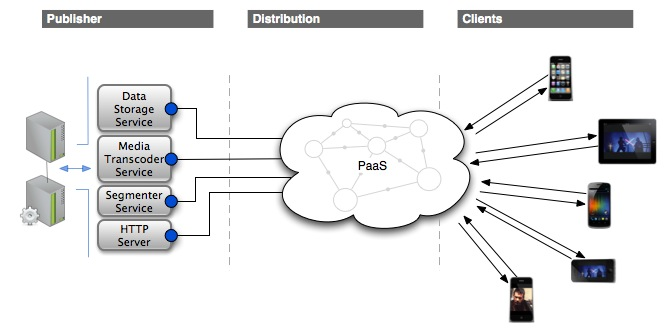
\includegraphics[width=0.9\textwidth]{./Images/cashed5}
%\caption{Ecosystem}
%\label{fig:cashed}
%\end{figure}
%
%Proin auctor lorem at nibh. Curabitur nulla purus, feugiat id, elementum in, lobortis quis, pede. Vivamus sodales adipiscing sapien. Vestibulum posuere nulla eget wisi. Integer volutpat ligula eget enim. Suspendisse vitae arcu. Quisque pellentesque. Nullam consequat, sem vitae rhoncus tristique, mauris nulla fermentum est, bibendum ullamcorper sapien magna et quam. Sed dapibus vehicula odio. Proin bibendum gravida nisl. Fusce lorem. Phasellus sagittis, nulla in hendrerit laoreet, libero lacus feugiat urna, eget hendrerit pede magna vitae lorem. Praesent mauris Class aptent taciti sociosqu ad litora torquent per conubia nostra, per inceptos hymenaeos H.264\slash \ac{AVC} standard, sem vitae rhoncus tristique \ac{SVC} \cite{Fraunhofer-Heinrich-Hertz-Institute:2013fk,ISO:H-264} nulla in hendrerit laoreet, libero lacus feugiat urna, eget hendrerit pede magna vitae lorem.
%
%\textcolor{violet}{You can use in-paragraph lists with this construct for: 
%\begin{inparaenum}[(a)]
%\item first case;
%\item second case; and
%\item third case,
%\end{inparaenum}
%making the text organized and fluid.}
%
%Vivamus auctor leo vel dui. Aliquam erat volutpat. Phasellus nibh. Vestibulum ante ipsum primis in faucibus orci luctus et ultrices posuere cubilia Curae; Cras tempor. Morbi egestas, urna non consequat tempus, nunc arcu mollis enim, eu aliquam erat nulla non nibh. Duis consectetuer malesuada velit. Nam ante nulla, interdum vel, tristique ac, condimentum non, tellus. Proin ornare feugiat nisl. Suspendisse dolor nisl, ultrices at, eleifend vel, consequat at, dolor, morbi egestas, urna non consequat tempus, nunc arcu mollis enim, eu aliquam erat nulla non nibh.
%
%
%
%Maecenas elementum augue nec nisl. Proin auctor lorem at nibh. Curabitur nulla purus, feugiat id, elementum in, lobortis quis, pede. Vivamus sodales adipiscing sapien. Vestibulum posuere nulla eget wisi. Integer volutpat ligula eget enim. Suspendisse vitae arcu. Quisque pellentesque.